\section{Implementierung}
Nachdem sowohl das Konzept und das Vorgehen erarbeitet wurden, konnte mit der Implementierung begonnen werden. Hier wurde dokumentiert, wie die geplanten Konzepte umgesetzt wurden und welche Probleme es dabei gab.
\subsection{Anpassungen}
Zu Beginn der Anpassung wurde als Erstes die bestehende Software auf die Erweiterung angepasst. Dabei wurden als Erstes die beiden Bibliotheken: WebSocketpp und die damit verbundene Asio Bibliothek hinzugefügt. Danach wurde mit den Änderungen begonnen. Der erste Schritt war es viele Funktionen im Code zu verändern, die davor nur auf die Impulsschnittstelle angepasst waren.\newline

\noindent Um die zukünftige Implementierung weiterer Schnittstellen einfacher zu gestalten wurden neben bereits definierten Schnittstellenarten: IMPULSE, OCPP1.6 und OCPP2.0.1, mit eingeplant, dass weitere hinzukommen könnten. Deshalb wurden die Schnittstellen Arten über ein \verb|enum| deklariert. Ergänzend zu den bereits genannten Typen, wurde ebenfalls der Typ \textit{Unknown} mit aufgenommen. Der Schnittstellen Typ \textit{Unknown} dient zu Fehlererkennung und ist invalide. Um die Funktionen anzupassen wurde in jeder Funktion, die zuvor nur nach dem \spverb|hwChannel| unterschieden hat, jetzt zusätzlich die Schnittstellenart mit angegeben. Dadurch kann die Unterscheidung nach dem \spverb|hwChannel| beim Schnittstellentyp \glqq{}IMPULSE\grqq{} immer noch erfolgen. Für die Ladesäulen wird zur Stationsunterscheidung, anstelle des \spverb|hwChannel|, das neu definierte Feld: \spverb|chargingPointNumber| genutzt. Damit können alle Stationstypen und Anschlüsse unterschieden werden. 
\subsection{GUI}
Nachdem alle Funktionen angepasst wurden, konnte die neue Stationsauswahl integriert werden. Hierfür wurde die bereits existierende Kilometer Stand Eingabe als Basis genommen. Hier mussten die angezeigten Texte und Icons angepasst werden, damit sie zu der Ladesäulenauswahl passen. Die finale Anzeige ist in \autoref{fig:Ladestationsauswahl_GUI} zusehen. 
\begin{figure}[H]
	\centering
	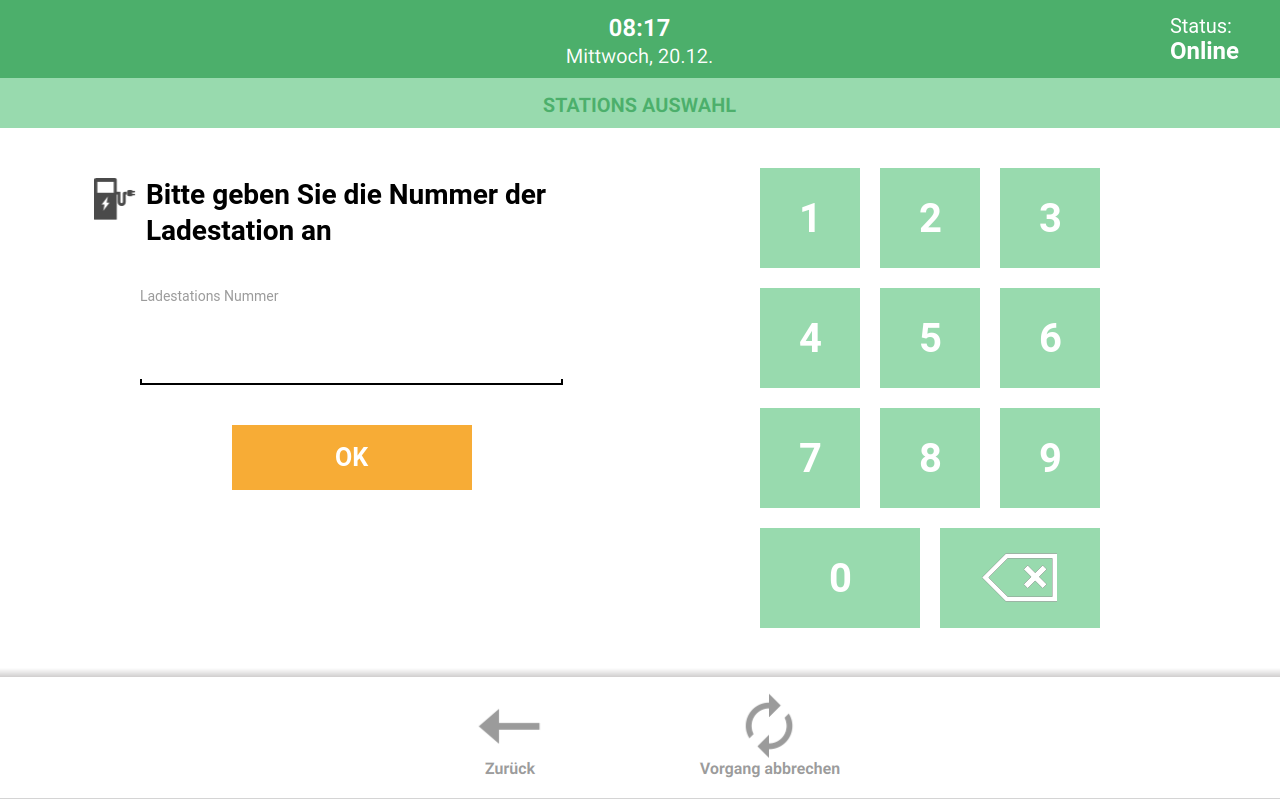
\includegraphics[width=1.0\textwidth]{images/GUI/LadestationsAuswahl.png}
	\caption{Ansicht bei der Auswahl einer Ladestation \cite{Konzept}}
	\label{fig:Ladestationsauswahl_GUI}
\end{figure}
\noindent Um die Ladesäulen Eingabe zu überprüfen wird über alle Stationen mit dem Schnittstellentyp OCPP1.6 oder OCPP2.0.1 in der Datenbank iteriert. Sollte keiner dieser Einträge die gesuchte \verb|chargingPointNumber| bzw. die eingegebene Nummer beinhalten, wird ein Fehlertext auf dem Bildschirm sichtbar. Nach dem zum dritten Mal eine ungültige \verb|chargingPointNumber| eingegeben wurde, wird der Startbildschirm angezeigt und der Fahrer muss sich erneut authentifizieren. Bei der korrekten Auswahl einer gültigen Ladesäule wird zuerst überprüft, ob an dieser ein Fahrzeug angeschlossen ist. Ist ein Fahrzeug angeschlossen, wird überprüft, ob dort bereits ein Ladevorgang aktiv ist. Erst wenn kein Ladevorgang an dem gewählten Anschluss aktiv ist, wird ein neuer gestartet. Sollte dazwischen eine dieser Bedingungen nicht erfüllt sein, wird eine Fehlermeldung angezeigt und der Fehlerzähler erhöht.\newline

\noindent Nachdem die Stationsauswahl implementiert wurde, konnte sich um die Produktauswahl gekümmert werden. Normalerweise wird für jeden Stationseintrag in der Datenbank eine entsprechende Kachel in der Produktauswahl angezeigt. Dieses Verhalten ist in \autoref{fig:Produktauswahl_GUI} zu sehen.

\begin{figure}[H]
	\centering
	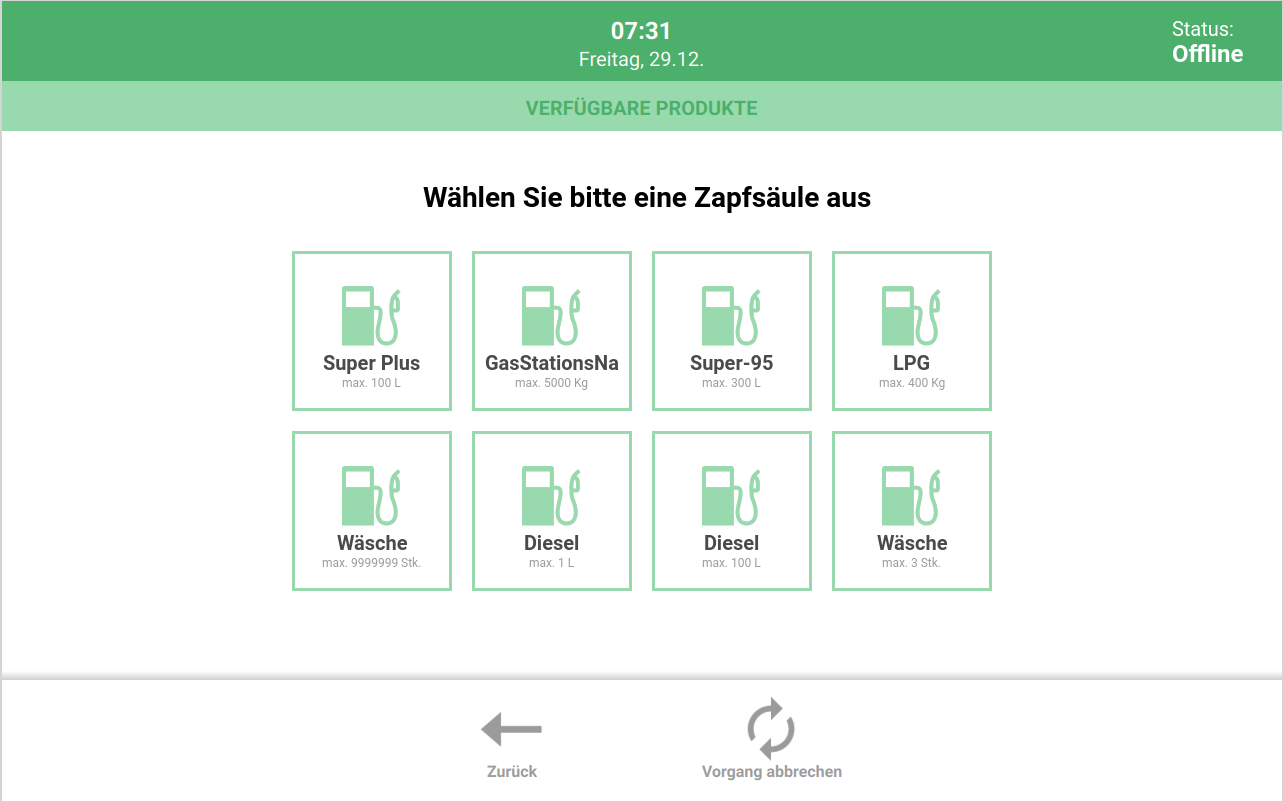
\includegraphics[width=1.0\textwidth]{images/GUI/Produktauswahl.PNG}
	\caption{Ansicht der Produktauswahl mit acht klassischen Stationen \cite{Konzept}}
	\label{fig:Produktauswahl_GUI}
\end{figure}

\noindent Da allerdings die Kachelansicht beibehalten werden möchte und es nun möglich ist mehr als die bisher vorgesehen acht Stationen anzuzeigen, musste eine andere Lösung gefunden werden.\\
\noindent Hierfür wurde eine allgemeine Kachel mit der Bezeichnung \glqq{}E-Ladestationen\grqq{} hinzugefügt. Sollte nun min. eine Ladesäule konfiguriert sein, wird diese angezeigt. Sollten mehrere Einträge existieren, wird weiterhin nur die beschriebene Kachel für alle weiteren Ladesäulen angezeigt. Sollte die Kachel jetzt ausgewählt werden, wird die Stationsauswahl aufgerufen. Um dieses Verhalten zu erzielen, wurden alle andere konfigurierten Ladesäulen ausgeblendet und nur die erste gefundene angezeigt. Außerdem wurde dafür gesorgt, dass die \glqq{}E-Ladestationen\grqq{} Kachel immer als letztes Element in der Produktauswahl angezeigt wird, um die Kachel Formatierung beizubehalten.

\subsection{OCPP Protokoll}
Nachdem die GUI Funktionen integriert wurden, konnten die einzelnen Aspekte des OCPP Protokolls integriert werden. Hierbei wurden die in \autoref{fig:Komponenten_Aufbau} gezeigten Komponenten umgesetzt, in dem aus diesen eigenen Klassen erstellt wurden.
\subsubsection{WebSocketServer}
%Noch run, start und senden beschreiben
Die WebsocketServer Klasse wurde mithilfe der WebSocketpp Bibliothek erstellt. In der \verb|run()| Methode der Klasse wird der zweite Thread gestartet und es wird auf eingehende Verbindungen/Nachrichten gewartet. Um auf die empfangenen Daten einzugehen wurden drei Callback Funktionen entworfen, die je nach Event von der Bibliothek aufgerufen werden (vgl.\cite{websocketpp_faq}, \glqq{}Handler Reference\grqq{}):
\begin{itemize}
	\item \verb|validate_handler|: Dieses Event wird ausgelöst, sobald ein WebSocket Handshake empfangen wurde, aber noch bevor dieser akzeptiert wird. In der dabei aufgerufenen Methode wird überprüft, ob sich der Client mit dem Server verbinden darf. Hierfür wird die mitgesendete \acs{URI} mit der \spverb|chargePointId| der Datenbankeinträge verglichen. Dasselbe wird für das WebSocket Subprotokoll getan.
	\item \verb|message_received_handler|: Der Handler wird, aufgerufen, sobald eine neue Nachricht über die geöffneten WebSocket Verbindungen empfangen wurde und stellt diese als String zur weiteren Verarbeitung bereit. Dabei wird ebenfalls der zur Ladesäule gehörende Datenbankeintrag ausgesucht und weitergegeben.
	\item \verb|close_handler|: Sobald ein Client die Verbindung schließt/verliert, wird das \textit{close Event} aufgerufen. Hier werden alle mit dem Client in Verbindung stehenden Daten entfernt und die WebSocket Verbindung auch Serverseitig geschlossen.
\end{itemize}

\noindent Zum Versenden der eigenen Daten wurde ebenfalls eine separate Methode eingeführt, die die Daten an eine angegebene Ladesäule mit der Methode \verb|send| sendet. Die korrekte Ladesäule wird aus einer Liste mit allen offenen WebSocket Verbindung ausgesucht. Dies geschieht unter der Angabe der \verb|chargePointId|. Welche aufgrund des Datenbankeintrags, auf die \spverb|chargepointNumber| zurückgeführt werden kann.

\subsubsection{RPC Protokoll}
Die RPC Klasse verarbeitet die im \verb|message_received_handler| empfangenen Daten. Hierfür wird der vom WebSocketServer übergebene String genutzt, um zu entscheiden, ob es sich um eine Call, CallResult oder CallError Nachricht handelt. \newline

\noindent Handelt es sich um eine Call Nachricht, wird aus dem übergebenen String die OCPP Aktion ausgelesen und der Inhalt an den OCPP Handler übergeben. Auf Basis des Feldes \glqq{}type\grqq{} im Datenbankeintrag, wird entschieden, ob der OCPP 1.6 oder 2.0.1 Handler aufgerufen wird.\newline

\noindent Wird eine CallResult Nachricht empfangen, ist das Vorgehen ähnlich. Hier wird die OCPP Aktion bestimmt, in dem diese aus einem Objekt ausgelesen wird. Das Objekt wird vor dem Versenden der dazu gehörenden Call Nachricht erstellt und bis zum Empfangen der CallResult Nachricht gespeichert. In diesem ist die zuletzt gesendete Nachricht, der Datenbankeintrag und ein \spverb|QTimer| Objekt enthalten. Alle so erstellten Nachrichtenobjekte werden vor dem Versenden in einer Liste gespeichert. Jede versendete Nachricht hat dabei eine Zeitüberschreitung nach 30 Sekunden, die über das enthaltene \spverb|QTimer| Objekt gezählt wird. Läuft der Timer ab, wird die Nachricht erneut gesendet. Das Ganze wird dreimal wiederholt, danach wird eine Fehlermeldung ausgegeben.\\
\noindent Beim Empfangen der CallResult Nachricht wird das Nachrichtenobjekt aus der Liste entfernt und die benötigten Parameter entnommen. Danach wird das Objekt gelöscht. Mit den Informationen kann jetzt der benötigte OCPP Nachrichten Handler aufgerufen werden. \newline

\noindent Sollte eine CallError Nachricht empfangen werden, kann wieder aus dem Nachrichtenobjekt alle benötigen Informationen genommen werden. Diesmal wird allerdings auf Basis des \verb|errorCode| der Nachricht eine Fehlermeldung in eine Logdatei geschrieben. Je nach Fehler Code wird dieselbe Call Nachricht erneut versendet.\\

\noindent Um das RPC Framework ebenfalls als Schnittstelle zur restlichen Logik zu gestalten, wurden Signale für die Events:
\begin{itemize}
	\item \spverb|meterValuesReceived|: Fortschritt der Lademenge während eines Ladevorgangs
	\item \spverb|stopTransactionReceived|: Ladevorgang wurde gestoppt
	\item \spverb|connectorStatusChanged|: Status eines Anschlusses der Ladesäule hat sich verändert
\end{itemize}
Festgelegt. Beim Auslösen des Events \spverb|MeterValuesReceived| wird die im GUI angezeigte Lademenge aktualisiert. Die Lademenge wird anhand der Differenz zwischen dem absoluten Wert in der \spverb|StartTransaction|/\spverb|TransactionEvent(type = Started)| Nachricht und dem absoluten Wert innerhalb der \spverb|MeterValues|/\spverb|Trans- actionEvent(type = Updated)| kalkuliert.
Wird ein \spverb|StopTransactionReceived| Event ausgelöst, wird der aktuell laufende Ladevorgang für den angegebenen Anschluss beendet und die finale Lademenge angezeigt. Dieses Event wird über die \spverb|StopTransaction|/\spverb|TransactionEvent(type = Ended)| Nachricht ausgelöst. Das \spverb|connectorStatusChanged| Event wird verwendet, um den gespeicherten Zustand der Ladesäule zu aktualisieren, also immer nachdem Empfangen der \spverb|StatusNotifi- cation|/\spverb|TransactionEvent(type = Updated)| Nachricht.
\subsubsection{OCPP Handler und Nachrichten}\label{OCPP Probleme Umsetzung}
Es wurden pro Protokollversion jeweils ein eigener OCPP Handler entworfen. Beide haben denselben Aufbau und besitzen Methoden zum Handhaben von Call und CallResult Nachrichten. Alle in \autoref{OCPP_Nachrcihten_bnoetigt} ermittelten Nachrichten wurden implementiert. Dabei sind alle Nachrichten, die vom Tankautomat versendet werden, in dem CallResult Handler und alle Nachrichten, die von der Ladesäule versendet werden, im Call Handler enthalten. Um zwischen den Nachrichten zu unterscheiden, wurde ein \spverb|switch-case| genutzt und für jede Nachricht ein eigener \spverb|case| angelegt. In diesem kann das beschriebene Nachrichtenobjekt angelegt werden und mit diesem dann weitergearbeitet werden.\\

\noindent Die einzelnen Nachrichten Klassen agieren dabei alle gleich. Sie überprüfen in der \spverb|process_XXX| Methode, den Payload Inhalt und setzten einen entsprechenden RPC \spverb|errorCode| (\cite{OCPP-j-1.6-specification}, S.13f. \& \cite{OCPP-2.0.1-part4-ocpp-j-specification}, S.14), falls der Inhalt nicht dem erlaubten Format entspricht.\\

\noindent Da OCPP 2.0.1 viele eigene Datentypen definiert, wurden für diese ebenfalls eigene Klassen, nachdem selben Prinzip hinzugefügt. Das hatte den Vorteil, dass die Datentypen für unterschiedliche Nachrichten wieder verwendet werden konnten.\newline

\noindent Für den komplexeren Ablauf in der Bootphase der Ladesäule wurde eine \textit{state-machine} implementiert, um die einzelnen Bootstadien zu unterscheiden. Sobald die Ladesäule sich verbindet, wird dafür prinzipiell mit einer \spverb|BootNotification(status = Pending)| geantwortet und mit \spverb|GetConfiguration| die Konfigurationsparameter abgefragt. Wenn diese von den gewünschten Werten abweichen und veränderbar sind, werden sie mit \spverb|ChangeConfiguration| gesetzt. Dabei wurde für die Parameter: \spverb|StopTransactionOnEVSideDisconnect| und \spverb|MeterValueSampledData| festgelegt, dass diese dem erwarteten Wert entsprechen müssen und ansonsten der Boot abgelehnt wird. Ansonsten wird der Boot angenommen und es wird auf den Input eines Fahrers oder auf den Input der Ladesäule gewartet. \\

\noindent \textbf{Probleme}\newline
\noindent Während der Entwicklung sind hauptsächlich Probleme aufgrund der OCPP Version 2.0.1 aufgetreten. Dabei wurde während der manuellen Tests (siehe \autoref{Testergebnisse}) erkannt, dass die Nachrichten: \spverb|MeterValues| und \spverb|SecurityEvent- Notification| auch integriert werden müssen. Die \spverb|SecurityEventNotification| Nachricht wird nach einem Neustart der Ladesäule gesendet und die \spverb|MeterValues| Nachricht übertragt den Energiezählerstatus, während keine Transaktion an der Ladesäule aktiv ist. Da diese Nachrichten keine spezielle Behandlung erfordern und nur eine Bestätigung benötigen, konnten diese schnell und einfach hinzugefügt werden. Dasselbe betraf die Konfigurationsparameter. Hier mussten zusätzlich die Konfigurationsparameter: \spverb|TxStartPoint|, \spverb|TxStopPoint|, \spverb|SampledDataTxStarted- Measurands| und \spverb|SampledDataTxEndedMeasurands| gesetzt werden, um zu bestimmen, wann eine Transaktion gestartet/beendet werden soll und welche Messwerte dabei mitgesendet werden. Diese wurden nach der Empfehlung der OCPP Dokumentation so angepasst, dass sie dem Verhalten einer OCPP1.6 Ladesäule entsprechen(vgl. \cite{OCPP-2.0.1-part2-specification-edition2}, S.116ff.).
\subsection{Cloud Schnittstelle}
Als letztes konnte sich um den in C-01 beschriebene Online/Offline Status der Ladesäule gekümmert werden. Dieser wurde über einen Timer umgesetzt. Sollte im festgelegten Intervall keine Nachricht von der Ladesäule empfangen werden wird das Online/Offline Feld in der bereits existierenden Synchronisationsnachricht zu null gesetzt, andernfalls wird es zu eins gesetzt.\newline
\noindent Da bereits in der restlichen Logik Ladevorgänge gleich wie Tankvorgänge behandelt werden musste zur Erfüllung von C-02 keine gesonderten Schritte getroffen werden.
